%%%%%%%%%%%%%%%%%%%%%%%%%%%%%%%%%%%%%%%%%%%%%%%%%%%%%%%%%%%%%%%%%%%%%%%%%%%%%%%%%%%%%%%%%
%             template.tex                                                              %
%                                                                                       %
%            Author: Sergej Lewin 10/2008                                               %
%                                                                                       %    
% !!!Man braucht noch die Datei Ueb.sty (im gleichen Ordner wie die Hauptdatei)!!!      %
%%%%%%%%%%%%%%%%%%%%%%%%%%%%%%%%%%%%%%%%%%%%%%%%%%%%%%%%%%%%%%%%%%%%%%%%%%%%%%%%%%%%%%%%%
\documentclass[a4paper,11pt]{article}             % bestimmt das Aussehen eines Dokuments
\usepackage{Ueb}                                  % vordefinierte Makros
\usepackage{enumitem}
\usepackage{mathtools}
\usepackage{tikz}
\renewcommand{\labelenumi}{(\alph{enumi})}
\renewcommand{\labelenumii}{(\roman{enumii})}

%!!!!anpassen an das Betriebssystem!!!, um Umlaute zu verwenden
\usepackage[utf8]{inputenc}                      %Linux
%\usepackage[latin1]{inputenc}                    %Windows
%\usepackage[applemac]{inputenc}                  %Mac



%Namen und Matrikelnummern anpassen
%\zweinamen{Name1}{Matrikelnummer1}{Name2}{Matrikelnummer2} %2er Gruppen
\dreinamen{Alexander Neuwirth}{439218}{Leonhard Segger}{440145}{Jonathan Sigrist}{441760} %3er Gruppe

%Briefkastennummer anpassen. z. B. \briefkasten{104}
\briefkasten{}

%Termin der Uebungsgruppe und Raum anpassen z. B. \termin{Mo. 12-14 , SR2}
\termin{Fr. 08-10, SR217}

%Blattnummer anpassen z. B. \blatt{5}
\blatt{10}

\begin{document}
\Aufgabe{36}
Die Methode hat eine Laufzeit von $\mathcal O(n)$, da jedes Element genau einmal aufgerufen wird.

\Aufgabe{37}
\begin{enumerate}
\item 
\begin{enumerate}
\item
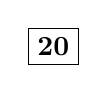
\begin{tikzpicture}[level/.style={sibling distance=30mm/#1}]
\node [rectangle,draw] {$\textbf{20}$};
\end{tikzpicture}

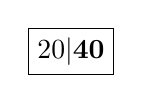
\begin{tikzpicture}[level/.style={sibling distance=30mm/#1}]
\node [rectangle,draw] {$20|\textbf{40}$};
\end{tikzpicture}

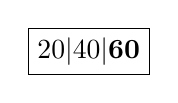
\begin{tikzpicture}[level/.style={sibling distance=30mm/#1}]
\node [rectangle,draw] {$20|40|\textbf{60}$};
\end{tikzpicture}

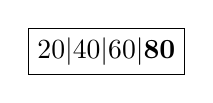
\begin{tikzpicture}[level/.style={sibling distance=30mm/#1}]
\node [rectangle,draw] {$20|40|60|\textbf{80}$};
\end{tikzpicture}

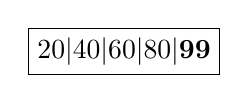
\begin{tikzpicture}[level/.style={sibling distance=30mm/#1}]
\node [rectangle,draw] {$20|40|60|80|\textbf{99}$};
\end{tikzpicture}

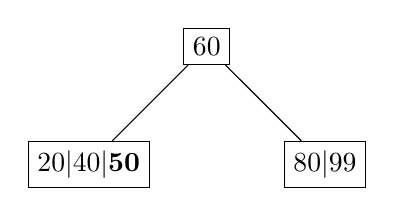
\begin{tikzpicture}[level/.style={sibling distance=30mm/#1}]
\node [rectangle,draw] {$60$}
  child {node[rectangle,draw] {$20|40|\textbf{50}$}}
  child {node[rectangle,draw] {$80|99$}}
;

\end{tikzpicture}

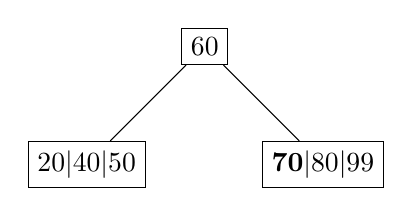
\begin{tikzpicture}[level/.style={sibling distance=30mm/#1}]
\node [rectangle,draw] {$60$}
  child {node[rectangle,draw] {$20|40|50$}}
  child {node[rectangle,draw] {$\textbf{70}|80|99$}}
;
\end{tikzpicture}

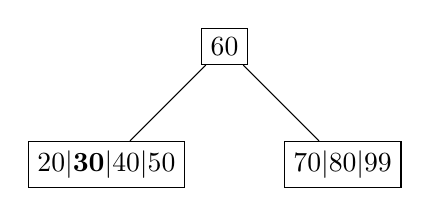
\begin{tikzpicture}[level/.style={sibling distance=30mm/#1}]
\node [rectangle,draw] {$60$}
  child {node[rectangle,draw] {$20|\textbf{30}|40|50$}}
  child {node[rectangle,draw] {$70|80|99$}}
;
\end{tikzpicture}

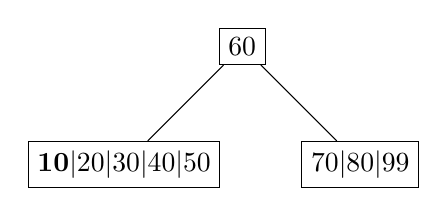
\begin{tikzpicture}[level/.style={sibling distance=30mm/#1}]
\node [rectangle,draw] {$60$}
  child {node[rectangle,draw] {$\textbf{10}|20|30|40|50$}}
  child {node[rectangle,draw] {$70|80|99$}}
;
\end{tikzpicture}

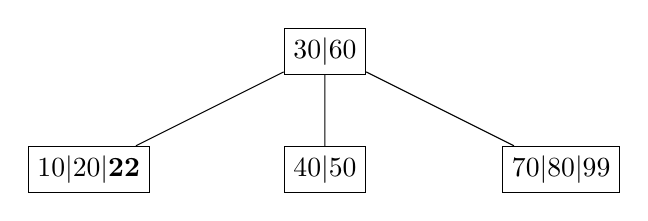
\begin{tikzpicture}[level/.style={sibling distance=30mm/#1}]
\node [rectangle,draw] {$30|60$}
  child {node[rectangle,draw] {$10|20|\textbf{22}$}}
  child {node[rectangle,draw] {$40|50$}}
  child {node[rectangle,draw] {$70|80|99$}}
;

\end{tikzpicture}

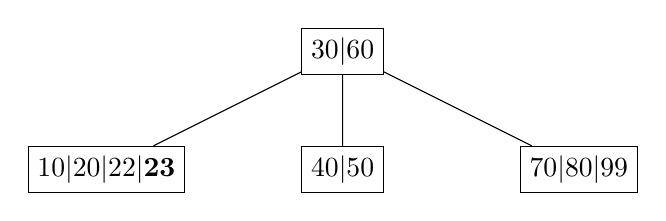
\begin{tikzpicture}[level/.style={sibling distance=30mm/#1}]
\node [rectangle,draw] {$30|60$}
  child {node[rectangle,draw] {$10|20|22|\textbf{23}$}}
  child {node[rectangle,draw] {$40|50$}}
  child {node[rectangle,draw] {$70|80|99$}}
;
\end{tikzpicture}

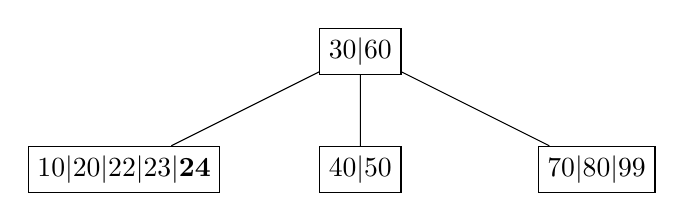
\begin{tikzpicture}[level/.style={sibling distance=30mm/#1}]
\node [rectangle,draw] {$30|60$}
  child {node[rectangle,draw] {$10|20|22|23|\textbf{24}$}}
  child {node[rectangle,draw] {$40|50$}}
  child {node[rectangle,draw] {$70|80|99$}}
;
\end{tikzpicture}

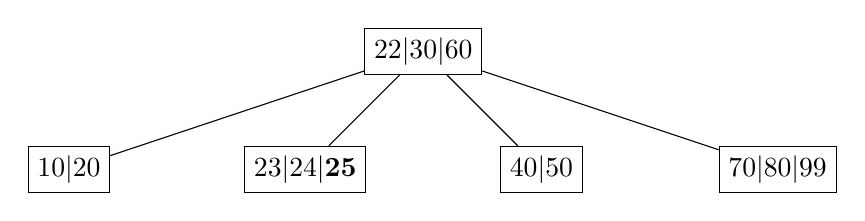
\begin{tikzpicture}[level/.style={sibling distance=30mm/#1}]
\node [rectangle,draw] {$22|30|60$}
  child {node[rectangle,draw] {$10|20$}}
  child {node[rectangle,draw] {$23|24|\textbf{25}$}}
  child {node[rectangle,draw] {$40|50$}}
  child {node[rectangle,draw] {$70|80|99$}}
;
\end{tikzpicture}

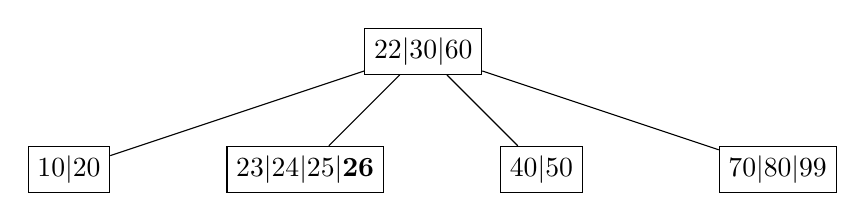
\begin{tikzpicture}[level/.style={sibling distance=30mm/#1}]
\node [rectangle,draw] {$22|30|60$}
  child {node[rectangle,draw] {$10|20$}}
  child {node[rectangle,draw] {$23|24|25|\textbf{26}$}}
  child {node[rectangle,draw] {$40|50$}}
  child {node[rectangle,draw] {$70|80|99$}}
;
\end{tikzpicture}

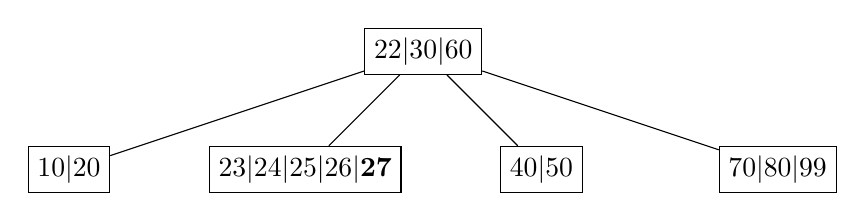
\begin{tikzpicture}[level/.style={sibling distance=30mm/#1}]
\node [rectangle,draw] {$22|30|60$}
  child {node[rectangle,draw] {$10|20$}}
  child {node[rectangle,draw] {$23|24|25|26|\textbf{27}$}}
  child {node[rectangle,draw] {$40|50$}}
  child {node[rectangle,draw] {$70|80|99$}}
;
\end{tikzpicture}

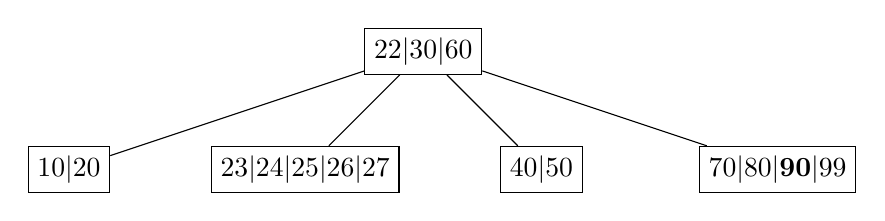
\begin{tikzpicture}[level/.style={sibling distance=30mm/#1}]
\node [rectangle,draw] {$22|30|60$}
  child {node[rectangle,draw] {$10|20$}}
  child {node[rectangle,draw] {$23|24|25|26|27$}}
  child {node[rectangle,draw] {$40|50$}}
  child {node[rectangle,draw] {$70|80|\textbf{90}|99$}}
;
\end{tikzpicture}

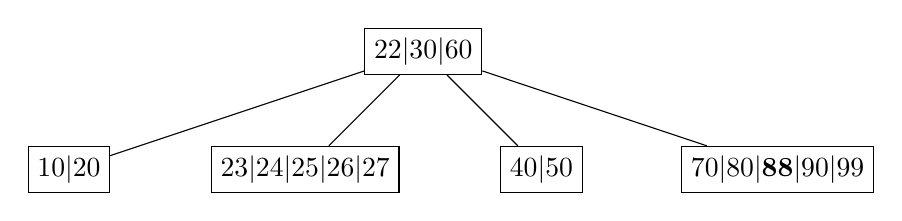
\begin{tikzpicture}[level/.style={sibling distance=30mm/#1}]
\node [rectangle,draw] {$22|30|60$}
  child {node[rectangle,draw] {$10|20$}}
  child {node[rectangle,draw] {$23|24|25|26|27$}}
  child {node[rectangle,draw] {$40|50$}}
  child {node[rectangle,draw] {$70|80|\textbf{88}|90|99$}}
;
\end{tikzpicture}

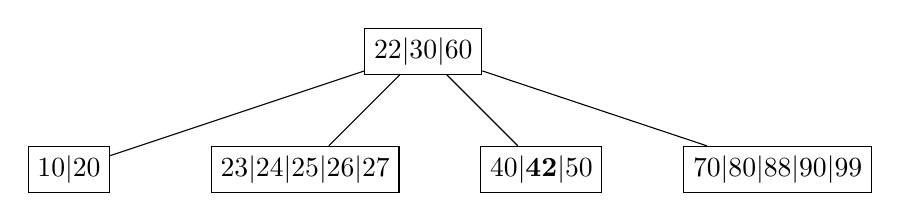
\begin{tikzpicture}[level/.style={sibling distance=30mm/#1}]
\node [rectangle,draw] {$22|30|60$}
  child {node[rectangle,draw] {$10|20$}}
  child {node[rectangle,draw] {$23|24|25|26|27$}}
  child {node[rectangle,draw] {$40|\textbf{42}|50$}}
  child {node[rectangle,draw] {$70|80|88|90|99$}}
;
\end{tikzpicture}

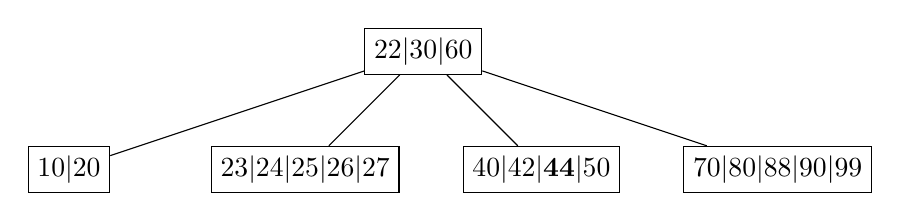
\begin{tikzpicture}[level/.style={sibling distance=30mm/#1}]
\node [rectangle,draw] {$22|30|60$}
  child {node[rectangle,draw] {$10|20$}}
  child {node[rectangle,draw] {$23|24|25|26|27$}}
  child {node[rectangle,draw] {$40|42|\textbf{44}|50$}}
  child {node[rectangle,draw] {$70|80|88|90|99$}}
;
\end{tikzpicture}

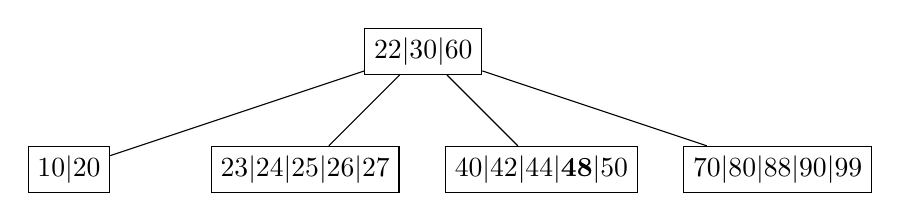
\begin{tikzpicture}[level/.style={sibling distance=30mm/#1}]
\node [rectangle,draw] {$22|30|60$}
  child {node[rectangle,draw] {$10|20$}}
  child {node[rectangle,draw] {$23|24|25|26|27$}}
  child {node[rectangle,draw] {$40|42|44|\textbf{48}|50$}}
  child {node[rectangle,draw] {$70|80|88|90|99$}}
;
\end{tikzpicture}

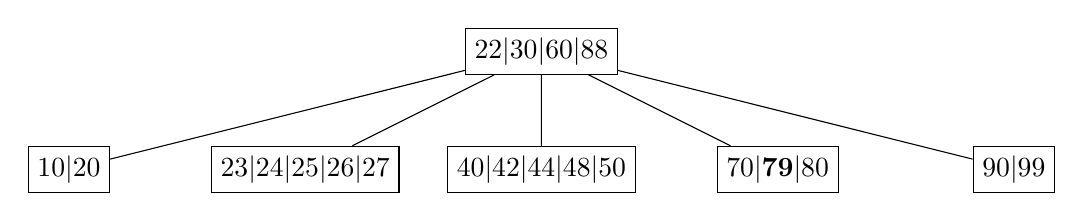
\begin{tikzpicture}[level/.style={sibling distance=30mm/#1}]
\node [rectangle,draw] {$22|30|60|88$}
  child {node[rectangle,draw] {$10|20$}}
  child {node[rectangle,draw] {$23|24|25|26|27$}}
  child {node[rectangle,draw] {$40|42|44|48|50$}}
  child {node[rectangle,draw] {$70|\textbf{79}|80$}}
  child {node[rectangle,draw] {$90|99$}}

;
\end{tikzpicture}

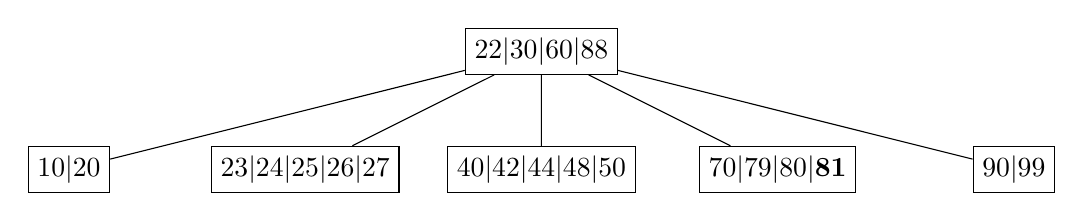
\begin{tikzpicture}[level/.style={sibling distance=30mm/#1}]
\node [rectangle,draw] {$22|30|60|88$}
  child {node[rectangle,draw] {$10|20$}}
  child {node[rectangle,draw] {$23|24|25|26|27$}}
  child {node[rectangle,draw] {$40|42|44|48|50$}}
  child {node[rectangle,draw] {$70|79|80|\textbf{81}$}}
  child {node[rectangle,draw] {$90|99$}}

;
\end{tikzpicture}

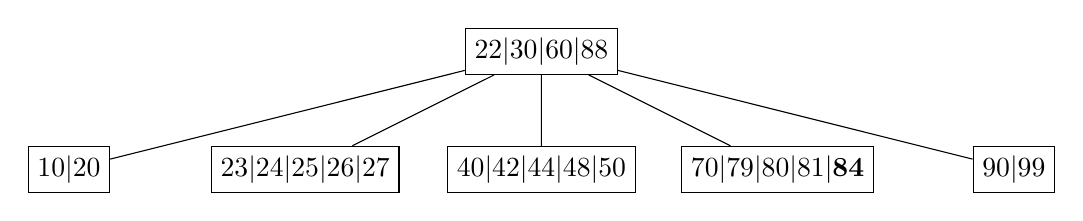
\begin{tikzpicture}[level/.style={sibling distance=30mm/#1}]
\node [rectangle,draw] {$22|30|60|88$}
  child {node[rectangle,draw] {$10|20$}}
  child {node[rectangle,draw] {$23|24|25|26|27$}}
  child {node[rectangle,draw] {$40|42|44|48|50$}}
  child {node[rectangle,draw] {$70|79|80|81|\textbf{84}$}}
  child {node[rectangle,draw] {$90|99$}}

;
\end{tikzpicture}

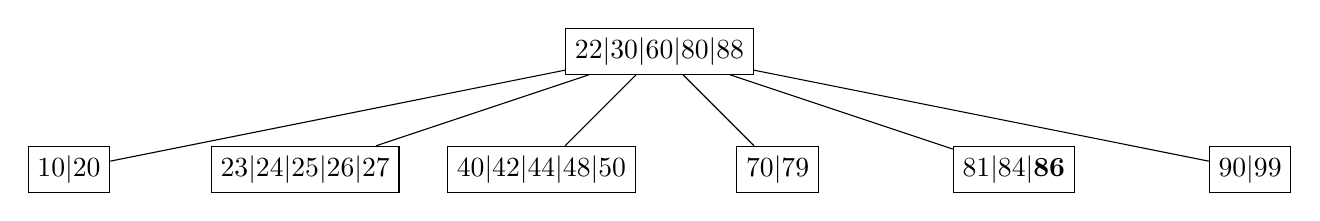
\begin{tikzpicture}[level/.style={sibling distance=30mm/#1}]
\node [rectangle,draw] {$22|30|60|80|88$}
  child {node[rectangle,draw] {$10|20$}}
  child {node[rectangle,draw] {$23|24|25|26|27$}}
  child {node[rectangle,draw] {$40|42|44|48|50$}}
  child {node[rectangle,draw] {$70|79$}}
  child {node[rectangle,draw] {$81|84|\textbf{86}$}}
  child {node[rectangle,draw] {$90|99$}}

;
\end{tikzpicture}

\item 

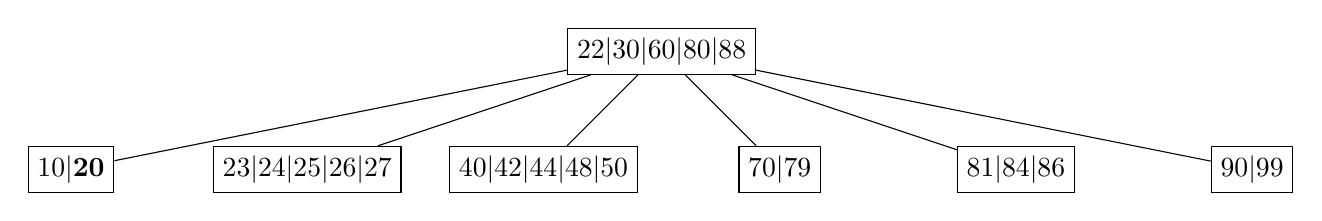
\begin{tikzpicture}[level/.style={sibling distance=30mm/#1}]
\node [rectangle,draw] {$22|30|60|80|88$}
  child {node[rectangle,draw] {$10|\textbf{20}$}}
  child {node[rectangle,draw] {$23|24|25|26|27$}}
  child {node[rectangle,draw] {$40|42|44|48|50$}}
  child {node[rectangle,draw] {$70|79$}}
  child {node[rectangle,draw] {$81|84|86$}}
  child {node[rectangle,draw] {$90|99$}}

;
\end{tikzpicture}

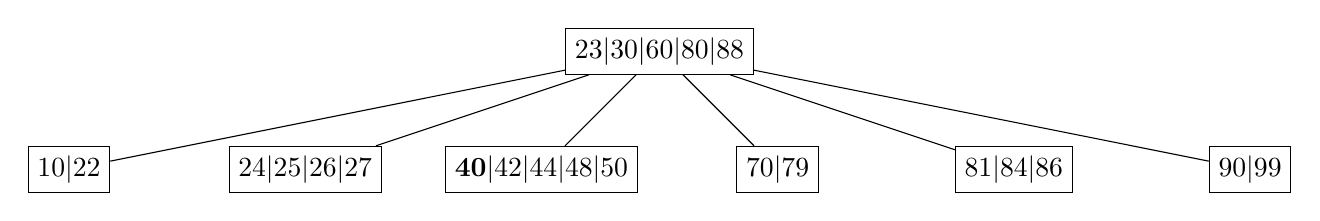
\begin{tikzpicture}[level/.style={sibling distance=30mm/#1}]
\node [rectangle,draw] {$23|30|60|80|88$}
  child {node[rectangle,draw] {$10|22$}}
  child {node[rectangle,draw] {$24|25|26|27$}}
  child {node[rectangle,draw] {$\textbf{40}|42|44|48|50$}}
  child {node[rectangle,draw] {$70|79$}}
  child {node[rectangle,draw] {$81|84|86$}}
  child {node[rectangle,draw] {$90|99$}}

;
\end{tikzpicture}

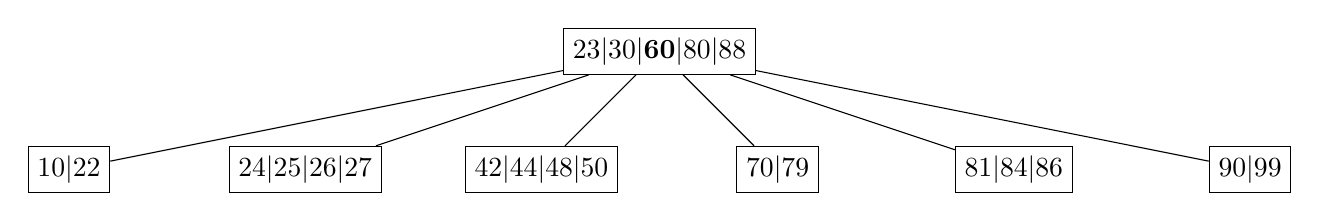
\begin{tikzpicture}[level/.style={sibling distance=30mm/#1}]
\node [rectangle,draw] {$23|30|\textbf{60}|80|88$}
  child {node[rectangle,draw] {$10|22$}}
  child {node[rectangle,draw] {$24|25|26|27$}}
  child {node[rectangle,draw] {$42|44|48|50$}}
  child {node[rectangle,draw] {$70|79$}}
  child {node[rectangle,draw] {$81|84|86$}}
  child {node[rectangle,draw] {$90|99$}}

;
\end{tikzpicture}

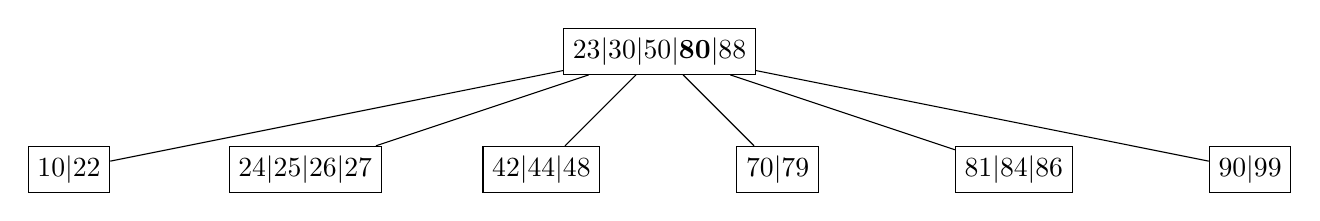
\begin{tikzpicture}[level/.style={sibling distance=30mm/#1}]
\node [rectangle,draw] {$23|30|50|\textbf{80}|88$}
  child {node[rectangle,draw] {$10|22$}}
  child {node[rectangle,draw] {$24|25|26|27$}}
  child {node[rectangle,draw] {$42|44|48$}}
  child {node[rectangle,draw] {$70|79$}}
  child {node[rectangle,draw] {$81|84|86$}}
  child {node[rectangle,draw] {$90|99$}}

;
\end{tikzpicture}

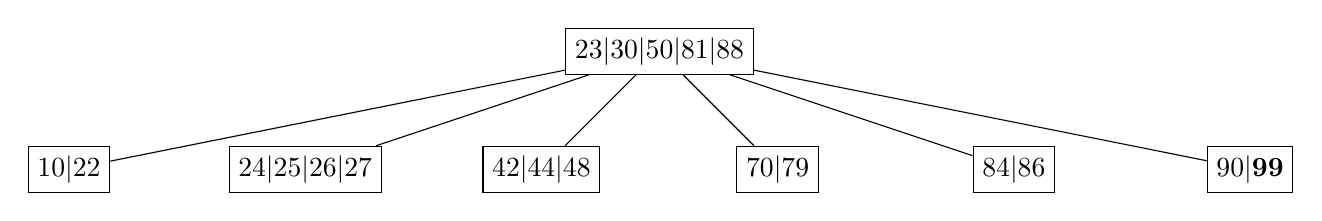
\begin{tikzpicture}[level/.style={sibling distance=30mm/#1}]
\node [rectangle,draw] {$23|30|50|81|88$}
  child {node[rectangle,draw] {$10|22$}}
  child {node[rectangle,draw] {$24|25|26|27$}}
  child {node[rectangle,draw] {$42|44|48$}}
  child {node[rectangle,draw] {$70|79$}}
  child {node[rectangle,draw] {$84|86$}}
  child {node[rectangle,draw] {$90|\textbf{99}$}}

;
\end{tikzpicture}

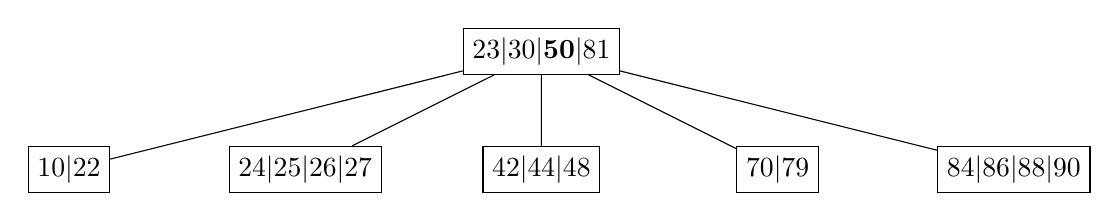
\begin{tikzpicture}[level/.style={sibling distance=30mm/#1}]
\node [rectangle,draw] {$23|30|\textbf{50}|81$}
  child {node[rectangle,draw] {$10|22$}}
  child {node[rectangle,draw] {$24|25|26|27$}}
  child {node[rectangle,draw] {$42|44|48$}}
  child {node[rectangle,draw] {$70|79$}}
  child {node[rectangle,draw] {$84|86|88|90$}}
;
\end{tikzpicture}

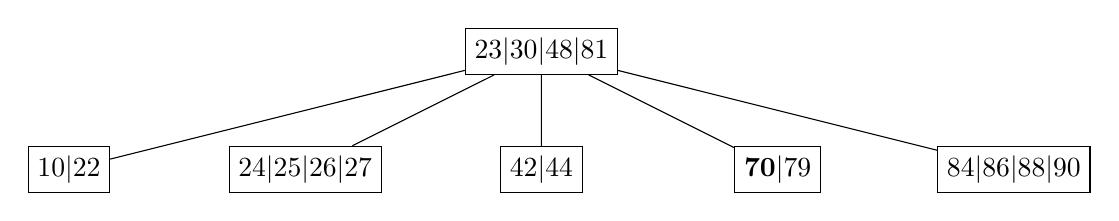
\begin{tikzpicture}[level/.style={sibling distance=30mm/#1}]
\node [rectangle,draw] {$23|30|48|81$}
  child {node[rectangle,draw] {$10|22$}}
  child {node[rectangle,draw] {$24|25|26|27$}}
  child {node[rectangle,draw] {$42|44$}}
  child {node[rectangle,draw] {$\textbf{70}|79$}}
  child {node[rectangle,draw] {$84|86|88|90$}}
;
\end{tikzpicture}

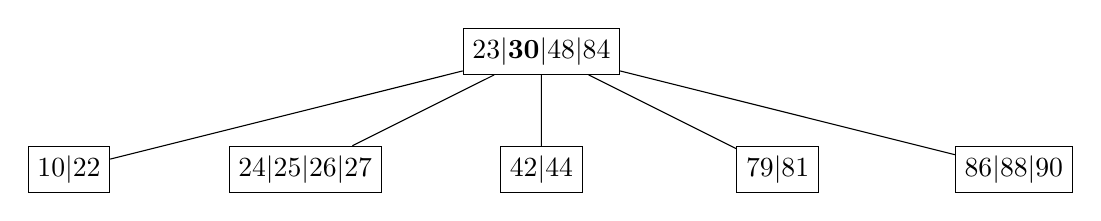
\begin{tikzpicture}[level/.style={sibling distance=30mm/#1}]
\node [rectangle,draw] {$23|\textbf{30}|48|84$}
  child {node[rectangle,draw] {$10|22$}}
  child {node[rectangle,draw] {$24|25|26|27$}}
  child {node[rectangle,draw] {$42|44$}}
  child {node[rectangle,draw] {$79|81$}}
  child {node[rectangle,draw] {$86|88|90$}}
;
\end{tikzpicture}

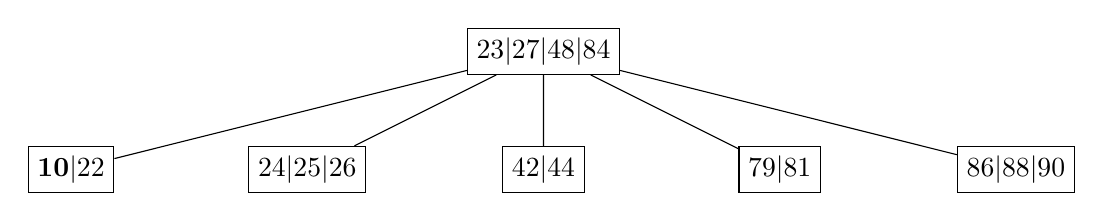
\begin{tikzpicture}[level/.style={sibling distance=30mm/#1}]
\node [rectangle,draw] {$23|27|48|84$}
  child {node[rectangle,draw] {$\textbf{10}|22$}}
  child {node[rectangle,draw] {$24|25|26$}}
  child {node[rectangle,draw] {$42|44$}}
  child {node[rectangle,draw] {$79|81$}}
  child {node[rectangle,draw] {$86|88|90$}}
;
\end{tikzpicture}

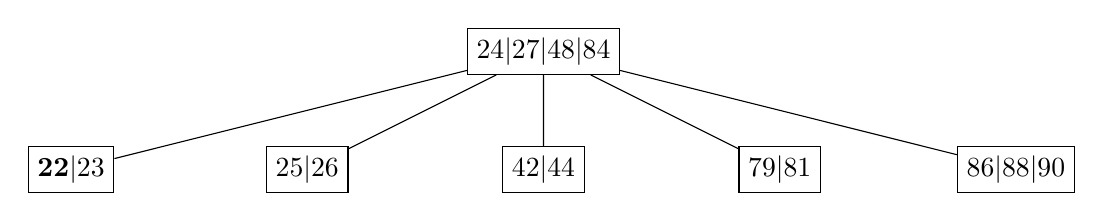
\begin{tikzpicture}[level/.style={sibling distance=30mm/#1}]
\node [rectangle,draw] {$24|27|48|84$}
  child {node[rectangle,draw] {$\textbf{22}|23$}}
  child {node[rectangle,draw] {$25|26$}}
  child {node[rectangle,draw] {$42|44$}}
  child {node[rectangle,draw] {$79|81$}}
  child {node[rectangle,draw] {$86|88|90$}}
;
\end{tikzpicture}

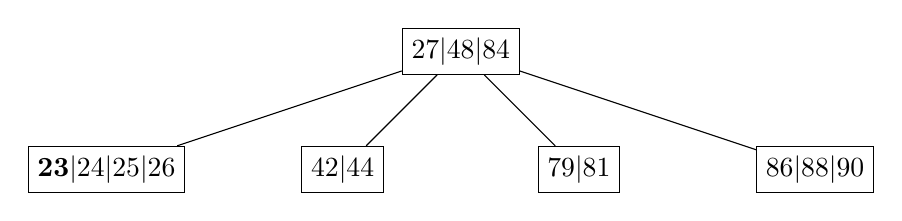
\begin{tikzpicture}[level/.style={sibling distance=30mm/#1}]
\node [rectangle,draw] {$27|48|84$}
  child {node[rectangle,draw] {$\textbf{23}|24|25|26$}}
  child {node[rectangle,draw] {$42|44$}}
  child {node[rectangle,draw] {$79|81$}}
  child {node[rectangle,draw] {$86|88|90$}}
;
\end{tikzpicture}

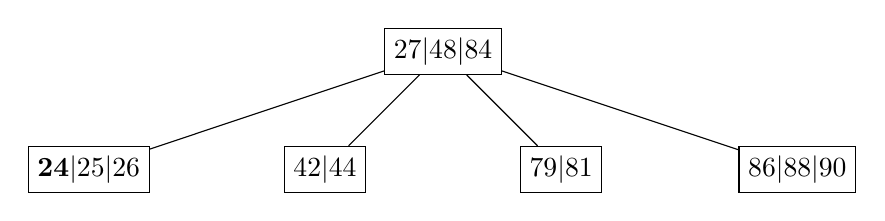
\begin{tikzpicture}[level/.style={sibling distance=30mm/#1}]
\node [rectangle,draw] {$27|48|84$}
  child {node[rectangle,draw] {$\textbf{24}|25|26$}}
  child {node[rectangle,draw] {$42|44$}}
  child {node[rectangle,draw] {$79|81$}}
  child {node[rectangle,draw] {$86|88|90$}}
;
\end{tikzpicture}

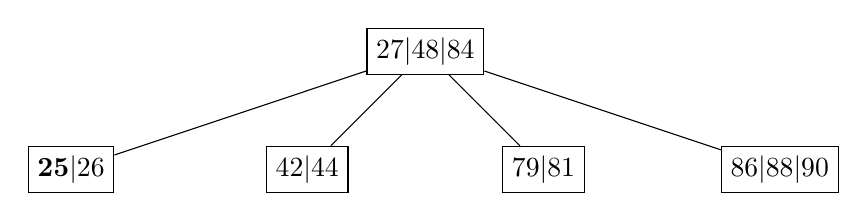
\begin{tikzpicture}[level/.style={sibling distance=30mm/#1}]
\node [rectangle,draw] {$27|48|84$}
  child {node[rectangle,draw] {$\textbf{25}|26$}}
  child {node[rectangle,draw] {$42|44$}}
  child {node[rectangle,draw] {$79|81$}}
  child {node[rectangle,draw] {$86|88|90$}}
;
\end{tikzpicture}

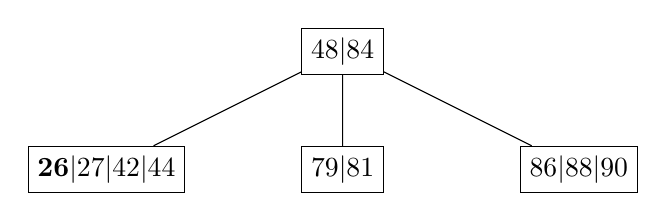
\begin{tikzpicture}[level/.style={sibling distance=30mm/#1}]
\node [rectangle,draw] {$48|84$}
  child {node[rectangle,draw] {$\textbf{26}|27|42|44$}}
  child {node[rectangle,draw] {$79|81$}}
  child {node[rectangle,draw] {$86|88|90$}}
;
\end{tikzpicture}

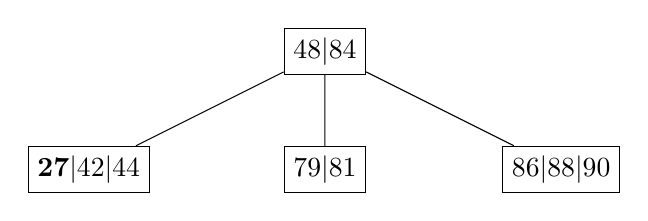
\begin{tikzpicture}[level/.style={sibling distance=30mm/#1}]
\node [rectangle,draw] {$48|84$}
  child {node[rectangle,draw] {$\textbf{27}|42|44$}}
  child {node[rectangle,draw] {$79|81$}}
  child {node[rectangle,draw] {$86|88|90$}}
;
\end{tikzpicture}

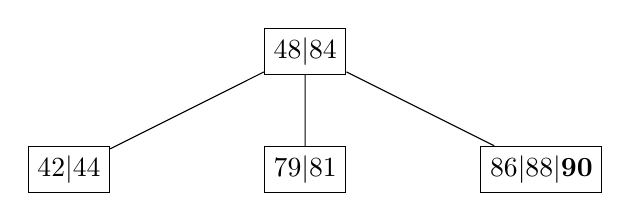
\begin{tikzpicture}[level/.style={sibling distance=30mm/#1}]
\node [rectangle,draw] {$48|84$}
  child {node[rectangle,draw] {$42|44$}}
  child {node[rectangle,draw] {$79|81$}}
  child {node[rectangle,draw] {$86|88|\textbf{90}$}}
;
\end{tikzpicture}

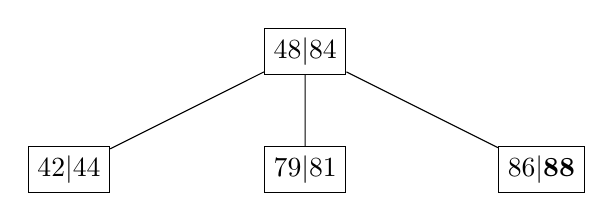
\begin{tikzpicture}[level/.style={sibling distance=30mm/#1}]
\node [rectangle,draw] {$48|84$}
  child {node[rectangle,draw] {$42|44$}}
  child {node[rectangle,draw] {$79|81$}}
  child {node[rectangle,draw] {$86|\textbf{88}$}}
;
\end{tikzpicture}

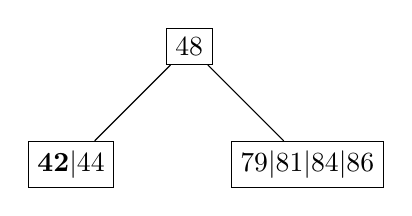
\begin{tikzpicture}[level/.style={sibling distance=30mm/#1}]
\node [rectangle,draw] {$48$}
  child {node[rectangle,draw] {$\textbf{42}|44$}}
  child {node[rectangle,draw] {$79|81|84|86$}}
;
\end{tikzpicture}

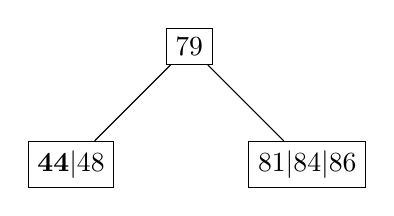
\begin{tikzpicture}[level/.style={sibling distance=30mm/#1}]
\node [rectangle,draw] {$79$}
  child {node[rectangle,draw] {$\textbf{44}|48$}}
  child {node[rectangle,draw] {$81|84|86$}}
;
\end{tikzpicture}

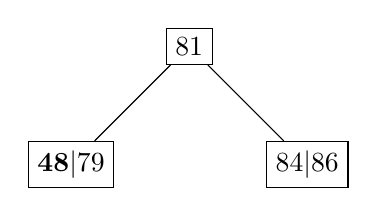
\begin{tikzpicture}[level/.style={sibling distance=30mm/#1}]
\node [rectangle,draw] {$81$}
  child {node[rectangle,draw] {$\textbf{48}|79$}}
  child {node[rectangle,draw] {$84|86$}}
;
\end{tikzpicture}

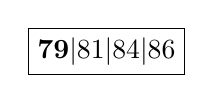
\begin{tikzpicture}[level/.style={sibling distance=30mm/#1}]
\node [rectangle,draw] {$\textbf{79}|81|84|86$};
\end{tikzpicture}

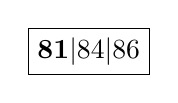
\begin{tikzpicture}[level/.style={sibling distance=30mm/#1}]
\node [rectangle,draw] {$\textbf{81}|84|86$};
\end{tikzpicture}

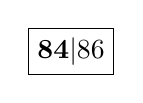
\begin{tikzpicture}[level/.style={sibling distance=30mm/#1}]
\node [rectangle,draw] {$\textbf{84}|86$};
\end{tikzpicture}

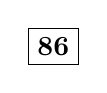
\begin{tikzpicture}[level/.style={sibling distance=30mm/#1}]
\node [rectangle,draw] {$\textbf{86}$};
\end{tikzpicture}
\end{enumerate}

\item
\begin{enumerate}
\item
\begin{description}
\item[1.Fall: $\mathcal B$ ist Blatt] Der Vorgänger ist der linke Nachbar von $\mathcal B$. Falls dieser nicht existiert, ist der Vorgänger der linke Vaterknoten. Falls auch dieser niht existiert, so wiederholt sich dieser Prozess für den Vaterknoten des Vaterknotens und so weiter. Also ist der erste (d. h. $n$ kleinst möglich) linke $n$-fache-Vaterknoten ist der Vorgänger. (außer Minimum)

Der Nachfolger ist dementsprechend der rechte Nachbar. Falls dieser nicht existiert, so ist der rechte Vaterknoten der Nachfolger und so weiter. Also ist der erste ($n$ kleinst möglich) rechte $n$-fache Vaterknoten der Nachfolger. (außer Maximum)

\item[2.Fall: $\mathcal B$ ist innerer Knoten] Vorgänger ist das Maximum des rechten Kinderknotens. Nachfolger das Minimum des linken Kinderknotens.

\item[Laufzeit:] Das Finden des $\mathcal B$-Elementes braucht $\mathcal O(\log n)$. Da die Position des Maximums bzw. des Minimums eines Teilbaums bekannt ist, beträgt die Laufzeit dafür $\mathcal O(1)$. Im Worst-Case muss der Baum bis zur Wurzel ($\mathcal O(\log n)$) geprüft werden, danach ist der Vorgänger/Nachfolger mit $\mathcal O(1)$ bekannt. Es folgt eine gesammte Laufzeit von $\mathcal O(\log n)$ für die Bestimmung von Vorgänger und Nachfolger.
\end{description}

\item
Jeder Knoten enthält zusätzlich einen Speicher für Vorgänger und Nachfolger. Falls nun ein neues Element eingefügt wird, werden Vorgänger und Nachfolger dessen bestimmt und deren Speicher des Nachfolgers bzw. des Vorgängers auf das neue Element gesetzt. Auch diese Operation braucht $\mathcal O(\log n)$.

Beim Löschen lassen sich die Nachfolger und Vorgänger des zu löschenden Elements auch mit $\mathcal O(\log n)$ bestimmen und deren Vorgänger- bzw. Nachfolgervariablen auf einander verweisen lassen. Somit hat auch diese Operation noch eine Laufzeit von $\mathcal O(\log n0)$.

Vorgänger und Nachfolger lassen sich nun mit $\mathcal O(1)$ bestimmen.
\end{enumerate}
\end{enumerate}

\Aufgabe{38}
$\xrightarrow{\text{insert 4}}$
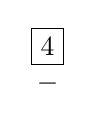
\begin{tikzpicture}[level/.style={sibling distance=30mm/#1}]
\node [label=below:$-$] [rectangle,draw] {$4$};
\end{tikzpicture}

$\xrightarrow{\text{insert 3}}$
\begin{tikzpicture}[level/.style={sibling distance=30mm/#1}]
\node [label=below:$\diagup$] [rectangle,draw] {$4$}
  child {node [label=below:$-$] [rectangle,draw] {$3$}}
  child {node {};}
;
\end{tikzpicture}

$\xrightarrow{\text{insert 2}}$
\begin{tikzpicture}[level/.style={sibling distance=30mm/#1}]
\node [label=below:$\diagup$] [rectangle,draw] {$4$}
  child {node [label=below:$\diagup$] [rectangle,draw] {$3$}
    child {node [label=below:$-$] [rectangle,draw] {$2$}}
    child {node {};}
  }
  child {node {};}
;
\end{tikzpicture}
$\xrightarrow{\text{Rotation}}$
\begin{tikzpicture}[level/.style={sibling distance=30mm/#1}]
\node [label=below:$-$] [rectangle,draw] {$3$}
  child {node [label=below:$-$] [rectangle,draw] {$2$}}
  child {node [label=below:$-$] [rectangle,draw] {$4$}}
;
\end{tikzpicture}

$\xrightarrow{\text{insert 1}}$
\begin{tikzpicture}[level/.style={sibling distance=30mm/#1}]
\node [label=below:$\diagup$] [rectangle,draw] {$3$}
  child {node [label=below:$\diagup$] [rectangle,draw] {$2$}
    child {node [label=below:$-$] [rectangle,draw] {$1$}}
    child {node {};}
  }
  child {node [label=below:$-$] [rectangle,draw] {$4$}}
;
\end{tikzpicture}

$\xrightarrow{\text{insert 8}}$
\begin{tikzpicture}[level/.style={sibling distance=30mm/#1}]
\node [label=below:$-$] [rectangle,draw] {$3$}
  child {node [label=below:$\diagup$] [rectangle,draw] {$2$}
    child {node [label=below:$-$] [rectangle,draw] {$1$}}
    child {node {};}
  }
  child {node [label=below:$\diagdown$] [rectangle,draw] {$4$}
    child {node {};}
    child {node [label=below:$-$] [rectangle,draw] {$8$}}
  }
;
\end{tikzpicture}

$\xrightarrow{\text{insert 7}}$
\begin{tikzpicture}[level/.style={sibling distance=30mm/#1}]
\node [label=below:$\diagdown$] [rectangle,draw] {$3$}
  child {node [label=below:$\diagup$] [rectangle,draw] {$2$}
    child {node [label=below:$-$] [rectangle,draw] {$1$}}
    child {node {};}
  }
  child {node [label=below:$\diagdown$] [rectangle,draw] {$4$}
    child {node {};}
    child {node [label=below:$\diagup$] [rectangle,draw] {$8$}
      child {node [label=below:$-$] [rectangle,draw] {$7$}}
      child {node {};}
    }
  }
;
\end{tikzpicture}
$\xrightarrow{\text{Doppelrotation}}$
\begin{tikzpicture}[level/.style={sibling distance=30mm/#1}]
\node [label=below:$-$] [rectangle,draw] {$3$}
  child {node [label=below:$\diagup$] [rectangle,draw] {$2$}
    child {node [label=below:$-$] [rectangle,draw] {$1$}}
    child {node {};}
  }
  child {node [label=below:$-$] [rectangle,draw] {$7$}
    child {node [label=below:$-$] [rectangle,draw] {$4$}}
    child {node [label=below:$-$] [rectangle,draw] {$8$}}
  }
;
\end{tikzpicture}

$\xrightarrow{\text{insert 6}}$
\begin{tikzpicture}[level/.style={sibling distance=30mm/#1}]
\node [label=below:$\diagdown$] [rectangle,draw] {$3$}
  child {node [label=below:$\diagup$] [rectangle,draw] {$2$}
    child {node [label=below:$-$] [rectangle,draw] {$1$}}
    child {node {};}
  }
  child {node [label=below:$\diagup$] [rectangle,draw] {$7$}
    child {node [label=below:$\diagdown$] [rectangle,draw] {$4$}
      child {node {};}
      child {node [label=below:$-$] [rectangle,draw] {$6$}}
    }
    child {node [label=below:$-$] [rectangle,draw] {$8$}}
  }
;
\end{tikzpicture}

$\xrightarrow{\text{insert 5}}$
\begin{tikzpicture}[level/.style={sibling distance=30mm/#1}]
\node [label=below:$\diagdown$] [rectangle,draw] {$3$}
  child {node [label=below:$\diagup$] [rectangle,draw] {$2$}
    child {node [label=below:$-$] [rectangle,draw] {$1$}}
    child {node {};}
  }
  child {node [label=below:$\diagup$] [rectangle,draw] {$7$}
    child {node [label=below:$\diagdown$] [rectangle,draw] {$4$}
      child {node {};}
      child {node [label=below:$\diagup$] [rectangle,draw] {$6$}
        child {node [label=below:$-$] [rectangle,draw] {$5$}}
        child {node {};}
      }
    }
    child {node [label=below:$-$] [rectangle,draw] {$8$}}
  }
;
\end{tikzpicture}
$\xrightarrow{\text{Doppelrotation}}$
\begin{tikzpicture}[level/.style={sibling distance=30mm/#1}]
\node [label=below:$\diagdown$] [rectangle,draw] {$3$}
  child {node [label=below:$\diagup$] [rectangle,draw] {$2$}
    child {node [label=below:$-$] [rectangle,draw] {$1$}}
    child {node {};}
  }
  child {node [label=below:$\diagup$] [rectangle,draw] {$7$}
    child {node [label=below:$-$] [rectangle,draw] {$5$}
      child {node [label=below:$-$] [rectangle,draw] {$4$}}
      child {node [label=below:$-$] [rectangle,draw] {$6$}}
    }
    child {node [label=below:$-$] [rectangle,draw] {$8$}}
  }
;
\end{tikzpicture}

$\xrightarrow{\text{insert 0}}$
\begin{tikzpicture}[level/.style={sibling distance=30mm/#1}]
\node [label=below:$-$] [rectangle,draw] {$3$}
  child {node [label=below:$\diagup$] [rectangle,draw] {$2$}
    child {node [label=below:$\diagup$] [rectangle,draw] {$1$}
      child {node [label=below:$-$] [rectangle,draw] {$0$}}
      child {node {};}
    }
    child {node {};}
  }
  child {node [label=below:$\diagup$] [rectangle,draw] {$7$}
    child {node [label=below:$-$] [rectangle,draw] {$5$}
      child {node [label=below:$-$] [rectangle,draw] {$4$}}
      child {node [label=below:$-$] [rectangle,draw] {$6$}}
    }
    child {node [label=below:$-$] [rectangle,draw] {$8$}}
  }
;
\end{tikzpicture}
$\xrightarrow{\text{Rotation}}$
\begin{tikzpicture}[level/.style={sibling distance=30mm/#1}]
\node [label=below:$\diagdown$] [rectangle,draw] {$3$}
  child {node [label=below:$-$] [rectangle,draw] {$1$}
    child {node [label=below:$-$] [rectangle,draw] {$0$}}
    child {node [label=below:$-$] [rectangle,draw] {$2$}}
  }
  child {node [label=below:$\diagup$] [rectangle,draw] {$7$}
    child {node [label=below:$-$] [rectangle,draw] {$5$}
      child {node [label=below:$-$] [rectangle,draw] {$4$}}
      child {node [label=below:$-$] [rectangle,draw] {$6$}}
    }
    child {node [label=below:$-$] [rectangle,draw] {$8$}}
  }
;
\end{tikzpicture}

$\xrightarrow{\text{insert 9}}$
\begin{tikzpicture}[level/.style={sibling distance=30mm/#1}]
\node [label=below:$\diagdown$] [rectangle,draw] {$3$}
  child {node [label=below:$-$] [rectangle,draw] {$1$}
    child {node [label=below:$-$] [rectangle,draw] {$0$}}
    child {node [label=below:$-$] [rectangle,draw] {$2$}}
  }
  child {node [label=below:$-$] [rectangle,draw] {$7$}
    child {node [label=below:$-$] [rectangle,draw] {$5$}
      child {node [label=below:$-$] [rectangle,draw] {$4$}}
      child {node [label=below:$-$] [rectangle,draw] {$6$}}
    }
    child {node [label=below:$\diagdown$] [rectangle,draw] {$8$}
      child {node {};}
      child {node [label=below:$-$] [rectangle,draw] {$9$}}
    }
  }
;
\end{tikzpicture}

$\xrightarrow{\text{remove 9}}$
\begin{tikzpicture}[level/.style={sibling distance=30mm/#1}]
\node [label=below:$\diagdown$] [rectangle,draw] {$3$}
  child {node [label=below:$-$] [rectangle,draw] {$1$}
    child {node [label=below:$-$] [rectangle,draw] {$0$}}
    child {node [label=below:$-$] [rectangle,draw] {$2$}}
  }
  child {node [label=below:$\diagup$] [rectangle,draw] {$7$}
    child {node [label=below:$-$] [rectangle,draw] {$5$}
      child {node [label=below:$-$] [rectangle,draw] {$4$}}
      child {node [label=below:$-$] [rectangle,draw] {$6$}}
    }
    child {node [label=below:$-$] [rectangle,draw] {$8$}}
  }
;
\end{tikzpicture}

$\xrightarrow{\text{remove 0}}$
\begin{tikzpicture}[level/.style={sibling distance=30mm/#1}]
\node [label=below:$\diagdown$] [rectangle,draw] {$3$}
  child {node [label=below:$\diagdown$] [rectangle,draw] {$1$}
    child {node {};}
    child {node [label=below:$-$] [rectangle,draw] {$2$}}
  }
  child {node [label=below:$\diagup$] [rectangle,draw] {$7$}
    child {node [label=below:$-$] [rectangle,draw] {$5$}
      child {node [label=below:$-$] [rectangle,draw] {$4$}}
      child {node [label=below:$-$] [rectangle,draw] {$6$}}
    }
    child {node [label=below:$-$] [rectangle,draw] {$8$}}
  }
;
\end{tikzpicture}

$\xrightarrow{\text{remove 5}}$
\begin{tikzpicture}[level/.style={sibling distance=30mm/#1}]
\node [label=below:$\diagdown$] [rectangle,draw] {$3$}
  child {node [label=below:$\diagdown$] [rectangle,draw] {$1$}
    child {node {};}
    child {node [label=below:$-$] [rectangle,draw] {$2$}}
  }
  child {node [label=below:$\diagup$] [rectangle,draw] {$7$}
    child {node [label=below:$\diagdown$] [rectangle,draw] {$4$}
      child {node {};}
      child {node [label=below:$-$] [rectangle,draw] {$6$}}
    }
    child {node [label=below:$-$] [rectangle,draw] {$8$}}
  }
;
\end{tikzpicture}

$\xrightarrow{\text{remove 6}}$
\begin{tikzpicture}[level/.style={sibling distance=30mm/#1}]
\node [label=below:$-$] [rectangle,draw] {$3$}
  child {node [label=below:$\diagdown$] [rectangle,draw] {$1$}
    child {node {};}
    child {node [label=below:$-$] [rectangle,draw] {$2$}}
  }
  child {node [label=below:$-$] [rectangle,draw] {$7$}
    child {node [label=below:$-$] [rectangle,draw] {$4$}}
    child {node [label=below:$-$] [rectangle,draw] {$8$}}
  }
;
\end{tikzpicture}

$\xrightarrow{\text{remove 7}}$
\begin{tikzpicture}[level/.style={sibling distance=30mm/#1}]
\node [label=below:$-$] [rectangle,draw] {$3$}
  child {node [label=below:$\diagdown$] [rectangle,draw] {$1$}
    child {node {};}
    child {node [label=below:$-$] [rectangle,draw] {$2$}}
  }
  child {node [label=below:$\diagdown$] [rectangle,draw] {$4$}
    child {node {};}
    child {node [label=below:$-$] [rectangle,draw] {$8$}}
  }
;
\end{tikzpicture}

$\xrightarrow{\text{remove 8}}$
\begin{tikzpicture}[level/.style={sibling distance=30mm/#1}]
\node [label=below:$\diagup$] [rectangle,draw] {$3$}
  child {node [label=below:$\diagdown$] [rectangle,draw] {$1$}
    child {node {};}
    child {node [label=below:$-$] [rectangle,draw] {$2$}}
  }
  child {node [label=below:$-$] [rectangle,draw] {$4$}}
;
\end{tikzpicture}

$\xrightarrow{\text{remove 1}}$
\begin{tikzpicture}[level/.style={sibling distance=30mm/#1}]
\node [label=below:$-$] [rectangle,draw] {$3$}
  child {node [label=below:$-$] [rectangle,draw] {$2$}}
  child {node [label=below:$-$] [rectangle,draw] {$4$}}
;
\end{tikzpicture}

$\xrightarrow{\text{remove 2}}$
\begin{tikzpicture}[level/.style={sibling distance=30mm/#1}]
\node [label=below:$\diagdown$] [rectangle,draw] {$3$}
  child {node {};}
  child {node [label=below:$-$] [rectangle,draw] {$4$}}
;
\end{tikzpicture}

$\xrightarrow{\text{remove 3}}$
\begin{tikzpicture}[level/.style={sibling distance=30mm/#1}]
\node [label=below:$-$] [rectangle,draw] {$4$};
\end{tikzpicture}

\Aufgabe{39}
\begin{enumerate}
\item
\begin{enumerate}
\item
\begin{equation*}
\begin{array}{c|ccccccccc}
S  &0&1&2&3&4&5&6&7&8\\
\hline
1) & & & & & &5& & & \\
2) & &28& & & &5& & & \\
3) & &28\rightarrow 19& & & &5& & & \\
4) & &28\rightarrow 19& & & &5&15& & \\
5) & &28\rightarrow 19&20& & &5&15& & \\
6) & &28\rightarrow 19&20& & &5&15\rightarrow 33& & \\
7) & &28\rightarrow 19&20&12& &5&15\rightarrow 33& & \\
8) & &28\rightarrow 19&20&12& &5&15\rightarrow 33& &17\\
\end{array}
\end{equation*}

\item
\begin{equation*}
\begin{array}{c|ccccccccc}
S  &0&1&2&3&4&5&6&7&8\\
\hline
1) & & & & & &5& & & \\
2) & &28& & & &5& & & \\
3) & &28&19& & &5& & & \\
4) & &28&19& & &5&15& & \\
5) & &28&19&20& &5&15& & \\
6) & &28&19&20& &5&15&33& \\
7) & &28&19&20&12&5&15&33& \\
8) & &28&19&20&12&5&15&33&17\\
\end{array}
\end{equation*}

\item
\begin{equation*}
\begin{array}{c|ccccccccc}
S  &0&1&2&3&4&5&6&7&8\\
\hline
1) & & & & & &5& & & \\
2) & &28& & & &5& & & \\
3) & &28&19& & &5& & & \\
4) & &28&19& & &5&15& & \\
5) & &28&19&20& &5&15& & \\
6) & &28&19&20& &5&15&33& \\
7) & &28&19&20&12&5&15&33& \\
8) & &28&19&20&12&5&15&33&17\\
\end{array}
\end{equation*}

\item
\begin{equation*}
\begin{array}{c|ccccccccc}
S  &0&1&2&3&4&5&6&7&8\\
\hline
1) & & & & & &5& & & \\
2) & &28& & & &5& & & \\
3) & &28& &19& &5& & & \\
4) & &28& &19& &5&15& & \\
5) & &28&20&19& &5&15& & \\
6) & &28&20&19&33&5&15& & \\
7) & &28&20&19&33&5&15&12& \\
8) & &28&20&19&33&5&15&12&17\\
\end{array}
\end{equation*}
\end{enumerate}

\item
Zur Speicherung von 6 Elementen werden 3 Bits benötigt. Also $g(x) \rightarrow [0,7]$.
\begin{equation*}
\begin{array}{ccc}
23 & = & \texttt{0010111}\\
35 & = & \texttt{0100011}\\
56 & = & \texttt{0111000}\\
81 & = & \texttt{1010001}\\
86 & = & \texttt{1011011}\\
91 & = & \texttt{1011011}
\end{array}
\end{equation*}
Damit ergibt sich die Funktion $g(x) = \texttt{(x>>6) | (x \& 6)}$.
\end{enumerate}

\Aufgabe{40}
\begin{enumerate}
\setcounter{enumi}{1}
\item 
\begin{enumerate}
\item Die Elemente können beim Einfügen zu einer linearen Liste werden. Dann müsste jeder Knoten überprüft werden, also $2^32$ Zugriffe.
\item Da der schiefste AVL-Baum eine Höhe von $1.44 \cdot \log_2 n$ hat, müssen im Worst-Caseeben so viele Zugriffe erfolgen.
\item Ein B-Baum mit $b=255$ hat ebenso $a=128$. Somit folgt eine maximale Höhe von $\log_{128}\left(\frac{2^{32} + 1}{2}+1  \right)\geq$ Höhe im Worst-Case. Das sind gerade mal 5 Zugriffe auf Knoten.
\end{enumerate}
\end{enumerate}
\end{document}

